\documentclass[hidelinks]{article}
\usepackage[utf8]{inputenc}
\usepackage{float}
\usepackage[danish]{babel}
\usepackage{graphicx}
\usepackage{siunitx}
\usepackage[margin=1.25in]{geometry}
\usepackage{hyperref}
\usepackage{url}
\usepackage{csquotes}

\usepackage[
style=alphabetic,
backend=biber,
sorting=nyt
]{biblatex}

\addbibresource{references.bib}

\setlength\parindent{0pt}

\title{Labuge 9/10 - Mål bilers fart}
\author{Marcus Koschmieder Krogsgaard\\
\small Med hjælp fra Christian Ringsing, Mie Gravgaard Lassen og Veronika Mantzius Postgaard}
\date{09. november 2023, kl. 15:00}

\begin{document}

\maketitle

\newpage

\section{Formål}
Formålet med øvelsen var at måle farten af en række biler på en vejstrækning, præsentere disse data i et histogram og bestemme bilernes middelfart.

\section{Fremgangsmåde} \label{fremgangsmaade}
Bilernes fart blev målt i samarbejde med Christian Ringsing, Mie Gravgaard Lassen og Veronika Mantzius Postgaard.\\

Personen der skal foretage målingerne placeres midt imellem to tydelige markeringer på vejen (ved dette forsøg blev der benyttet to parkeringsbåse, se fig. \ref{fig:pplads}). Afstanden mellem markeringerne opmåles fra kanten af den ene markering til kanten af den anden.\\

Når en bils forhjul passerer hver markering, gemmes tidspunktet, hvor hjulet kørte over markeringen. Den første tid trækkes fra den anden og tiden bilen var om at krydse strækningen gemmes i en fil. Dette foregår vha. et Python-script\cite{timescript}. Bemærk at der ikke foretages målinger ved meget langsom eller stillestående trafik (køkørsel).\\

Følgende formel benyttes til at beregne bilernes fart:

\[v = \frac{l}{t}\]

hvor $l$ er afstanden mellem markeringerne og $t$ er tiden bilen var om at krydse strækningen.\\

Ved dette forsøg blev målingerne foretaget på Østerbrogade nær Trianglen, i retning mod Poul Henningsens Plads. Målingerne blev foretaget torsdag den 09.11.2023 i tidsrummet 15:00-17:00 og der blev i alt foretaget 243 målinger.\\

\begin{figure}[H]
    \centering
    \includegraphics[width = 0.5\textwidth]{img/pbåse.jpg}
    \caption{De to parkeringsbåse der blev benyttet som markeringer ved dette forsøg.}
    \label{fig:pplads}
\end{figure}

\newpage

\section{Databehandling}

\subsection{Systematiske usikkerheder}

Der er to systematiske usikkerheder ved dette forsøg, nemlig usikkerheden på målingen af tiden det tog bilerne at krydse strækningen og usikkerheden på længden af strækningen de krydsede.\\

Reaktionstiden af Marcus Koschmieder Krogsgaard, der foretog målingerne, vurderes til at være $\pm$ 0,2 s. Denne værdi er benyttet som usikkerheden på målingen af tiden det tog bilerne at krydse strækningen.\\

Bestemmelsen af hvornår en bils forhjul havde passeret hver markering foregik ved øjemål. Usikkerheden på længden af strækningen en given bil passerede vurderes derfor til at være $\pm$ 0,5 m (måleusikkerheden ved opmålingen af strækningen er tilstrækkeligt lille til at den ikke får nogen betydning).\\

\subsection{Usikkerhed på middelfarten af bilerne} \label{usikkerhedmiddelfart}

Usikkerheden på middelfarten af bilerne er bestemt ved hjælp af ophobningsloven:\\

\[\Delta_f = \sqrt{\sum_{i = 1}^{n} \left( \frac{\partial f}{\partial x_i} \cdot \Delta_{\alpha_i} \right)^2}\]

Da farten af en bil er givet ved $v = \frac{l}{t}$ giver dette:

\[\Delta_v = \sqrt{\left(\frac{1}{t}\right)^2 \cdot \Delta^2_l + \left(\frac{-l}{t^2}\right)^2 \cdot \Delta^2_t}\]

Usikkerheden på middelværdien af længden er den samme som den systematiske usikkerhed på længden, da længden af strækningen er den samme for alle biler. Usikkerheden på middelværdien af tiden er bestemt til at være $\pm$ 0.01 s.\\

Da middelfarten af bilerne er givet ved $v = \frac{l}{t}$, hvor $t$ er den gennemsnitlige tid det tog en bil at passere strækningen, indsættes middelværdien af tiden bilerne var om at passere strækningen i formlen fra ophobningsloven. Dette giver en usikkerhed på middelfarten af bilerne på $\pm$ 0,6 m/s svarende til $\pm$ 2 km/h.\\

Standardafvigelsen af farten af bilerne er bestemt til at være $\pm$ 5,69 km/h og middelfarten er bestemt til at være $(27 \pm 2)$ km/h. Histogrammet over bilernes fart ses på fig. \ref{fig:histogram}. \\

\subsection{Histogram}

\begin{figure}[H]
    \centering
    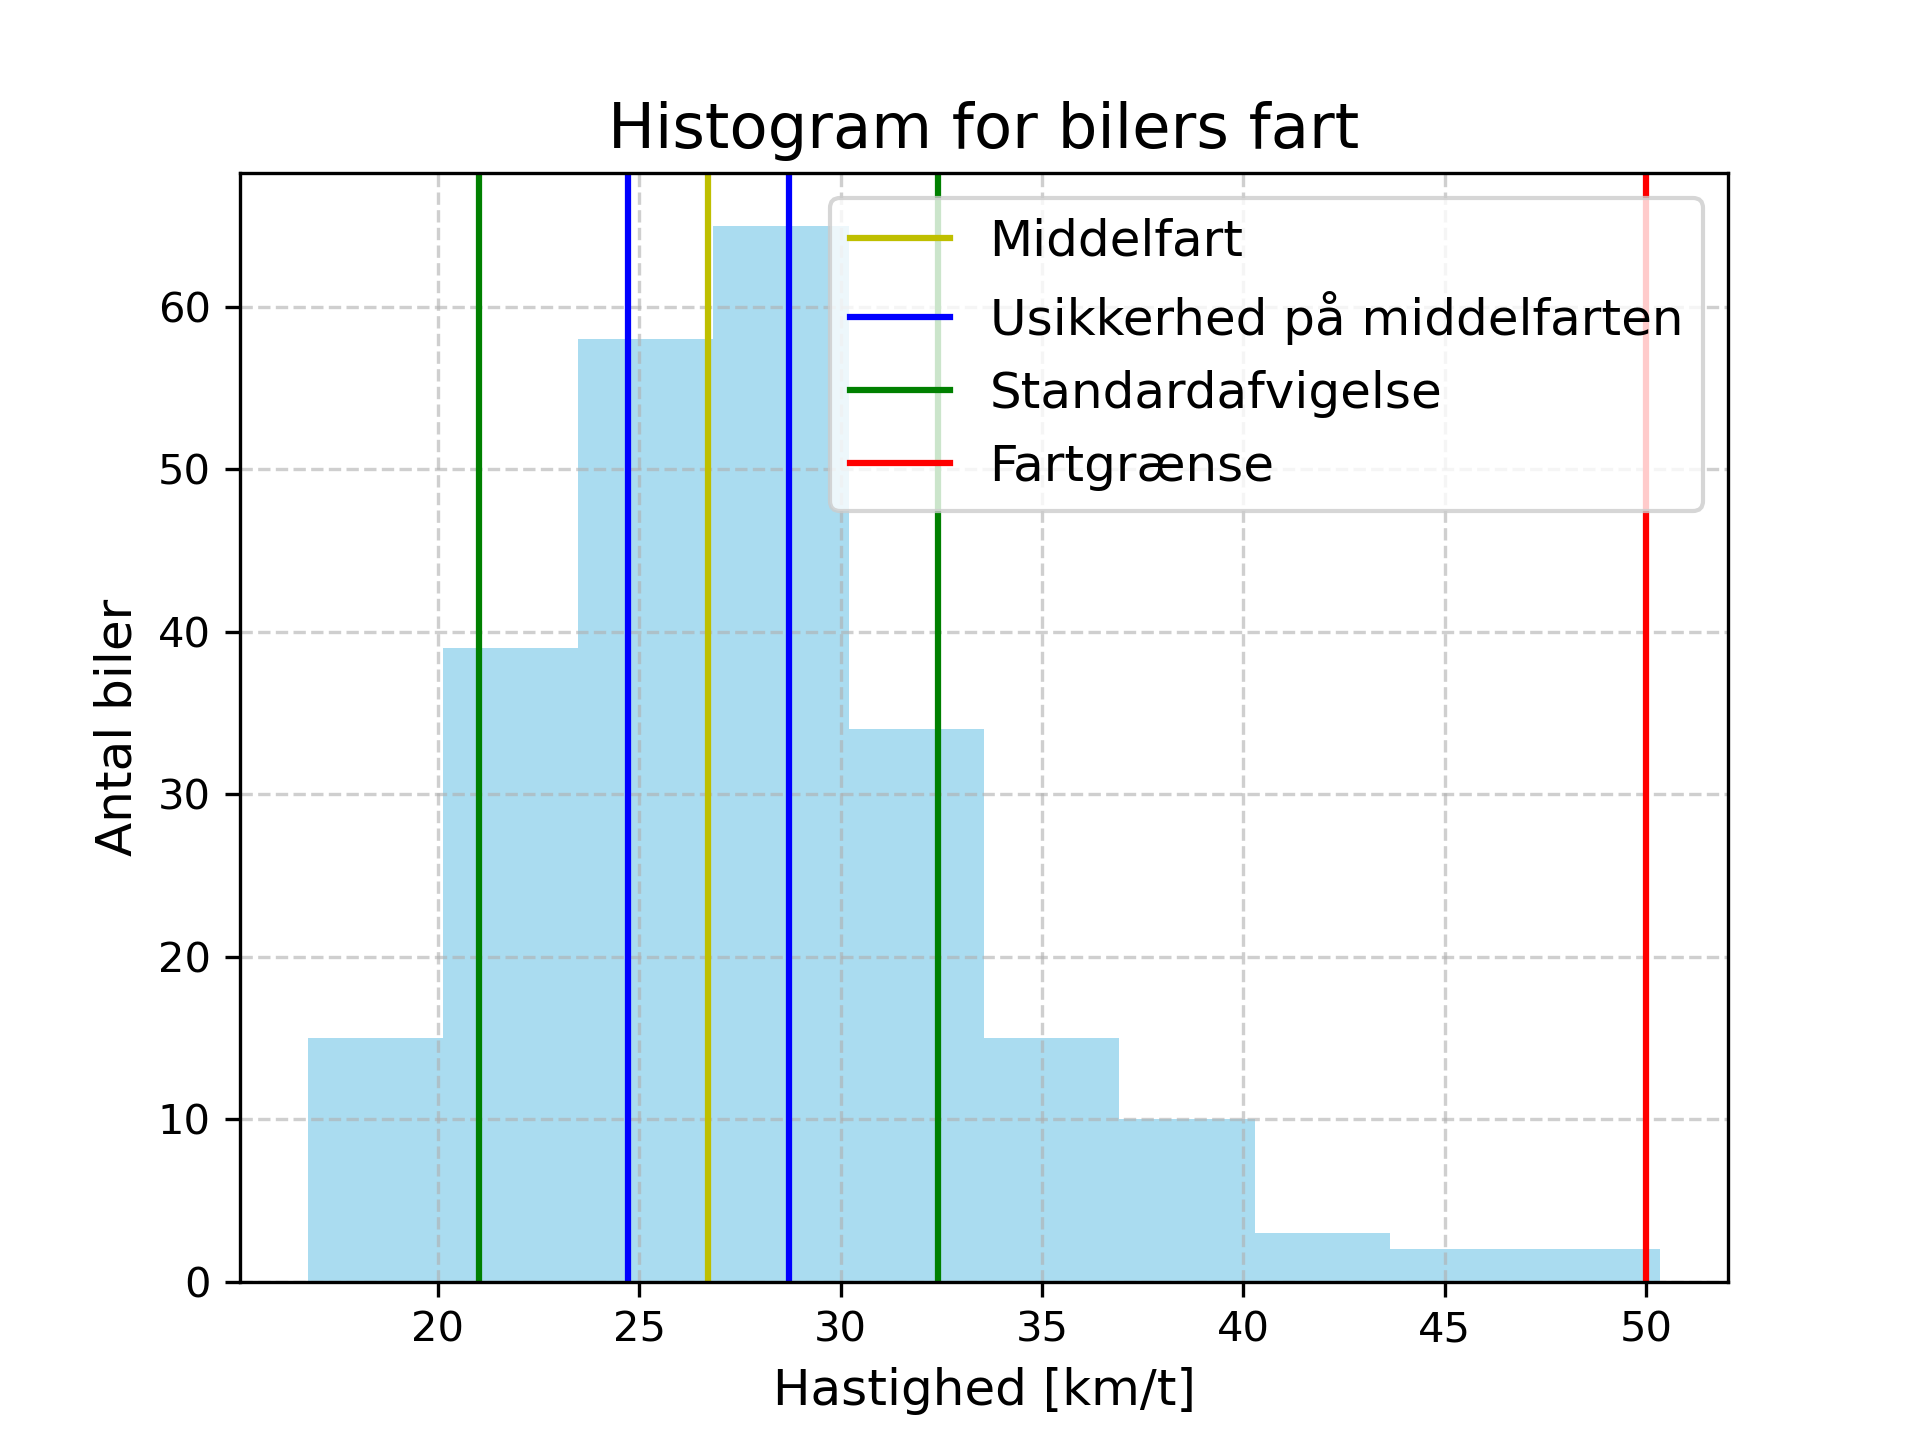
\includegraphics[width = 0.75 \textwidth]{img/histogram.png}
    \caption{Histogram over bilernes fart.}
    \label{fig:histogram}
\end{figure}

\section{Refleksion}

Histogrammet (fig. \ref{fig:histogram}) viser at bilernes fart er tilnærmelsesvist normalfordelt. Der lader dog til at være en række outliers der kørte relativt hurtigt i forhold til den gennemsnitlige bil.\\

Det er desuden tydeligt at der er en tendens til at bilerne kørte langt under fartgrænsen, hvilket giver god mening, da målingerne blev foretaget i myldretiden på en meget traffikeret vej. Det regnede også imens målingerne blev foretaget, hvilket nok har ført til endnu tættere trafik end normalt.\\

Med hensyn til usikkerheden på middelværdien af hastigheden er $\pm$ 2 km/h en relativt lille usikkerhed på under 10\% af middelværdien. Man kunne dog godt have ønsket sig en mindre usikkerhed, givet det store antal målinger. Størrelsen af usikkerheden skyldes den store systematiske usikkerhed på længden af strækningen og på tidsmålingerne. \\

Det fremgår af udtrykket for usikkerheden af middelværdien i sektion \ref{usikkerhedmiddelfart} at usikkerhed på tidsmålingerne vil få størst betydning og denne effekt vil være endnu mere væsentlig ved dette forsøg, grundet den meget korte afstand mellem markeringerne (og de tilsvarende korte tider).\\

Grundet fremgangsmåden i forsøget var det desværre ikke muligt at måle bilerne over en større strækning, da det ville blive meget svært at vurdere hvornår en bil havde passeret en markering. Man kunne derfor med rette spørge sig selv hvorfor vi ikke valgte en anden metode.\\

Vores gruppe på fire personer gennemførte faktisk forsøget tre gange. De første to gange benyttede vi en anden fremgangsmåde, hvor to personer stod i hver sin ende af en længere strækning og registrerede de tidspunkter biler passerede dem på. Til sidst blev tiderne sammenlignet og starttiderne trukket fra sluttiderne for at finde tiden bilerne var om at passere strækningen.\\

Desværre var der problemer med at synkronisere de to computere, dels fordi deres ur "tabte tid" i løbet af forsøget og der var forskelle i hvor hurtigt Python-scriptet gemte tiderne på de forskellige computere. Der var for mange faktorer der havde indflydelse på forsinkelsen (f.eks. hvor meget strøm computerne havde, hvilke programmer der var åbne i baggrunden og endda hvor koldt det var!) og da forsinkelsen varierede mellem hver måling var det svært at tage højde for den.\\

Disse forskelle viste sig til at være væsentlige nok til at gøre vores data ubrugelige. Uheldigvis gik det først op for os efter at vi havde foretaget ca. 300 målinger...\\

Denne metode havde en betydeligt laver usikkerhed på strækningen bilerne bevægede sig, da det var nemmere at vurdere hvornår en bil passerede observertøren når observertøren kiggede ligeud i stedet for at se på en markering der lå et stykke til siden for observatøren. Den systematiske usikkerhed på tiden var som sagt også mindre væsentlig idet længden af tidsintervallerne steg, mens usikkerheden var den samme som ved det endelige forsøg.\\

Det er derfor ærgerligt, at vi var nødt til at ændre vores fremgangsmåde til den der er beskrevet i sektion \ref{fremgangsmaade}.

\section{Konklusion}

Der blev foretaget 243 målinger med en systematisk usikkerhed på $\pm$ 0,5 m for længden af strækningen og $\pm$ 0,2 s for tiden bilerne var om at passere den.\\

Middelfarten af bilerne blev bestemt til $(27 \pm 2)$ km/h.

\section{Referencer}
\printbibliography[
heading=none
]

\end{document}
